% AgentMPI: A Message Passing Interface for Multi-Agent Systems
%
% Build:  latexmk -pdf main.tex     (or: pdflatex; bibtex; pdflatex; pdflatex)
% Numbers come from results.tex, generated by ../scripts/make_macros.py.
% Figures come from figures/, generated by ../scripts/figures.py.

\documentclass[10pt,twocolumn]{article}

\usepackage[T1]{fontenc}
\usepackage[utf8]{inputenc}
\usepackage{lmodern}
\usepackage[margin=0.85in]{geometry}
\usepackage{amsmath,amssymb}
\usepackage{graphicx}
\usepackage{booktabs}
\usepackage{tabularx}
\usepackage{multirow}
\usepackage{microtype}
\usepackage{xspace}
\usepackage{balance}
\usepackage[hyphens]{url}
\usepackage[hidelinks]{hyperref}
\usepackage{cleveref}
\usepackage{enumitem}
\usepackage{listings}
\usepackage{xcolor}
\usepackage{caption}

\captionsetup{font=small,labelfont=bf,skip=4pt}
\setlist{nosep,leftmargin=1.2em}

\definecolor{shell}{gray}{0.96}
\lstdefinestyle{shell}{
  basicstyle=\ttfamily\scriptsize,
  backgroundcolor=\color{shell},
  frame=single, framerule=0pt, framesep=3pt,
  breaklines=true, breakatwhitespace=true,
  columns=fullflexible, keepspaces=true,
  showstringspaces=false, xleftmargin=0pt, aboveskip=4pt, belowskip=4pt,
}
\lstset{style=shell}

\newcommand{\ampi}{\textsc{AgentMPI}\xspace}
\newcommand{\cli}[1]{\texttt{\small #1}}
\newcommand{\op}[1]{\texttt{\small #1}}

% Generated by scripts/make_macros.py from committed run data.
% Do not edit: every number here is computed from experiments/results/ or runs/.

\newcommand{\agHandlePeak}{5{,}080\xspace}
\newcommand{\agHandleTotal}{650{,}240\xspace}
\newcommand{\agInlinePeak}{508{,}000\xspace}
\newcommand{\agInlineTotal}{65{,}024{,}000\xspace}
\newcommand{\agPeakRatio}{100\xspace}
\newcommand{\alphaJournal}{3.947\xspace}
\newcommand{\alphaMemory}{0.096\xspace}
\newcommand{\alphaSqlite}{0.730\xspace}
\newcommand{\barCentraleight}{14\xspace}
\newcommand{\barCentralsixtyfour}{126\xspace}
\newcommand{\barCentraltwofiftysix}{510\xspace}
\newcommand{\barDissemeight}{24\xspace}
\newcommand{\barDissemsixtyfour}{384\xspace}
\newcommand{\barDissemtwofiftysix}{2{,}048\xspace}
\newcommand{\bestGammaThirty}{180.0\xspace}
\newcommand{\betaSpread}{1.5\xspace}
\newcommand{\betaSqlite}{0.480\xspace}
\newcommand{\confLines}{1{,}512\xspace}
\newcommand{\ctxN}{4{,}000\xspace}
\newcommand{\ctxP}{128\xspace}
\newcommand{\eLargeCtrlConsistency}{0.994\xspace}
\newcommand{\eLargeCtrlStrict}{0.9632\xspace}
\newcommand{\eLargeCtrlTokens}{24{,}406\xspace}
\newcommand{\eLargeCtrlWall}{255\xspace}
\newcommand{\eLargeExecutors}{8\xspace}
\newcommand{\eLargeGlossConsistency}{0.994\xspace}
\newcommand{\eLargeGlossStrict}{0.9509\xspace}
\newcommand{\eLargeGlossTokens}{26{,}480\xspace}
\newcommand{\eLargeGlossWall}{346\xspace}
\newcommand{\eLargeP}{32\xspace}
\newcommand{\eLargeTermsScored}{15\xspace}
\newcommand{\eLargeWallRatio}{1.4\xspace}
\newcommand{\eOneCtrlConsistency}{1.000\xspace}
\newcommand{\eOneCtrlStrict}{0.9474\xspace}
\newcommand{\eOneCtrlTokens}{6{,}082\xspace}
\newcommand{\eOneCtrlWall}{109\xspace}
\newcommand{\eOneExecutors}{16\xspace}
\newcommand{\eOneGlossConsistency}{1.000\xspace}
\newcommand{\eOneGlossStrict}{0.9474\xspace}
\newcommand{\eOneGlossTokens}{6{,}648\xspace}
\newcommand{\eOneGlossWall}{400\xspace}
\newcommand{\eOneP}{8\xspace}
\newcommand{\eOneTermsScored}{10\xspace}
\newcommand{\eOneVerdict}{healthy\xspace}
\newcommand{\eOneWallRatio}{3.7\xspace}
\newcommand{\eScaleConsistency}{0.994\xspace}
\newcommand{\eScaleContext}{\textit{n/a}\xspace}
\newcommand{\eScaleDisagree}{4\xspace}
\newcommand{\eScaleExecutors}{\textit{n/a}\xspace}
\newcommand{\eScaleOversub}{\textit{n/a}\xspace}
\newcommand{\eScaleRanks}{\textit{n/a}\xspace}
\newcommand{\eScaleStrict}{0.9509\xspace}
\newcommand{\eScaleSucceeded}{\textit{n/a}\xspace}
\newcommand{\eScaleTermsScored}{15\xspace}
\newcommand{\eScaleTokens}{\textit{n/a}\xspace}
\newcommand{\eScaleWall}{\textit{n/a}\xspace}
\newcommand{\eSixBlockedfour}{\textit{n/a}\xspace}
\newcommand{\eSixBlockedsixteen}{\textit{n/a}\xspace}
\newcommand{\eSixBlockedsixtyfour}{\textit{n/a}\xspace}
\newcommand{\eSixBlockedthirtytwo}{\textit{n/a}\xspace}
\newcommand{\eSixClaimAttemptsfour}{\textit{n/a}\xspace}
\newcommand{\eSixClaimAttemptssixteen}{\textit{n/a}\xspace}
\newcommand{\eSixClaimAttemptssixtyfour}{\textit{n/a}\xspace}
\newcommand{\eSixClaimAttemptsthirtytwo}{\textit{n/a}\xspace}
\newcommand{\eSixClaimsWonfour}{\textit{n/a}\xspace}
\newcommand{\eSixClaimsWonsixteen}{\textit{n/a}\xspace}
\newcommand{\eSixClaimsWonsixtyfour}{\textit{n/a}\xspace}
\newcommand{\eSixClaimsWonthirtytwo}{\textit{n/a}\xspace}
\newcommand{\eSixCommitsPerRankfour}{\textit{n/a}\xspace}
\newcommand{\eSixCommitsPerRanksixteen}{\textit{n/a}\xspace}
\newcommand{\eSixCommitsPerRanksixtyfour}{\textit{n/a}\xspace}
\newcommand{\eSixCommitsPerRankthirtytwo}{\textit{n/a}\xspace}
\newcommand{\eSixCommitsfour}{\textit{n/a}\xspace}
\newcommand{\eSixCommitssixteen}{\textit{n/a}\xspace}
\newcommand{\eSixCommitssixtyfour}{\textit{n/a}\xspace}
\newcommand{\eSixCommitsthirtytwo}{\textit{n/a}\xspace}
\newcommand{\eSixConffour}{\textit{n/a}\xspace}
\newcommand{\eSixConfsixteen}{\textit{n/a}\xspace}
\newcommand{\eSixConfsixtyfour}{\textit{n/a}\xspace}
\newcommand{\eSixConfthirtytwo}{\textit{n/a}\xspace}
\newcommand{\eSixConvictedfour}{\textit{n/a}\xspace}
\newcommand{\eSixConvictedsixteen}{\textit{n/a}\xspace}
\newcommand{\eSixConvictedsixtyfour}{\textit{n/a}\xspace}
\newcommand{\eSixConvictedthirtytwo}{\textit{n/a}\xspace}
\newcommand{\eSixCoordfour}{\textit{n/a}\xspace}
\newcommand{\eSixCoordsixteen}{\textit{n/a}\xspace}
\newcommand{\eSixCoordsixtyfour}{\textit{n/a}\xspace}
\newcommand{\eSixCoordthirtytwo}{\textit{n/a}\xspace}
\newcommand{\eSixEfffour}{\textit{n/a}\xspace}
\newcommand{\eSixEffsixteen}{\textit{n/a}\xspace}
\newcommand{\eSixEffsixtyfour}{\textit{n/a}\xspace}
\newcommand{\eSixEffthirtytwo}{\textit{n/a}\xspace}
\newcommand{\eSixExecutorsLostfour}{\textit{n/a}\xspace}
\newcommand{\eSixExecutorsLostsixteen}{\textit{n/a}\xspace}
\newcommand{\eSixExecutorsLostsixtyfour}{\textit{n/a}\xspace}
\newcommand{\eSixExecutorsLostthirtytwo}{\textit{n/a}\xspace}
\newcommand{\eSixExpectedfour}{\textit{n/a}\xspace}
\newcommand{\eSixExpectedsixteen}{\textit{n/a}\xspace}
\newcommand{\eSixExpectedsixtyfour}{\textit{n/a}\xspace}
\newcommand{\eSixExpectedthirtytwo}{\textit{n/a}\xspace}
\newcommand{\eSixLockWaitfour}{\textit{n/a}\xspace}
\newcommand{\eSixLockWaitsixteen}{\textit{n/a}\xspace}
\newcommand{\eSixLockWaitsixtyfour}{\textit{n/a}\xspace}
\newcommand{\eSixLockWaitthirtytwo}{\textit{n/a}\xspace}
\newcommand{\eSixMachinesfour}{\textit{n/a}\xspace}
\newcommand{\eSixMachinessixteen}{\textit{n/a}\xspace}
\newcommand{\eSixMachinessixtyfour}{\textit{n/a}\xspace}
\newcommand{\eSixMachinesthirtytwo}{\textit{n/a}\xspace}
\newcommand{\eSixPagesfour}{\textit{n/a}\xspace}
\newcommand{\eSixPagessixteen}{\textit{n/a}\xspace}
\newcommand{\eSixPagessixtyfour}{\textit{n/a}\xspace}
\newcommand{\eSixPagesthirtytwo}{\textit{n/a}\xspace}
\newcommand{\eSixParfour}{\textit{n/a}\xspace}
\newcommand{\eSixParsixteen}{\textit{n/a}\xspace}
\newcommand{\eSixParsixtyfour}{\textit{n/a}\xspace}
\newcommand{\eSixParthirtytwo}{\textit{n/a}\xspace}
\newcommand{\eSixResearchMedianfour}{\textit{n/a}\xspace}
\newcommand{\eSixResearchMediansixteen}{\textit{n/a}\xspace}
\newcommand{\eSixResearchMediansixtyfour}{\textit{n/a}\xspace}
\newcommand{\eSixResearchMedianthirtytwo}{\textit{n/a}\xspace}
\newcommand{\eSixResearchedfour}{\textit{n/a}\xspace}
\newcommand{\eSixResearchedsixteen}{\textit{n/a}\xspace}
\newcommand{\eSixResearchedsixtyfour}{\textit{n/a}\xspace}
\newcommand{\eSixResearchedthirtytwo}{\textit{n/a}\xspace}
\newcommand{\eSixReviewNfour}{\textit{n/a}\xspace}
\newcommand{\eSixReviewNsixteen}{\textit{n/a}\xspace}
\newcommand{\eSixReviewNsixtyfour}{\textit{n/a}\xspace}
\newcommand{\eSixReviewNthirtytwo}{\textit{n/a}\xspace}
\newcommand{\eSixReviseNfour}{\textit{n/a}\xspace}
\newcommand{\eSixReviseNsixteen}{\textit{n/a}\xspace}
\newcommand{\eSixReviseNsixtyfour}{\textit{n/a}\xspace}
\newcommand{\eSixReviseNthirtytwo}{\textit{n/a}\xspace}
\newcommand{\eSixScales}{0\xspace}
\newcommand{\eSixSentencesfour}{\textit{n/a}\xspace}
\newcommand{\eSixSentencessixteen}{\textit{n/a}\xspace}
\newcommand{\eSixSentencessixtyfour}{\textit{n/a}\xspace}
\newcommand{\eSixSentencesthirtytwo}{\textit{n/a}\xspace}
\newcommand{\eSixStolenfour}{\textit{n/a}\xspace}
\newcommand{\eSixStolensixteen}{\textit{n/a}\xspace}
\newcommand{\eSixStolensixtyfour}{\textit{n/a}\xspace}
\newcommand{\eSixStolenthirtytwo}{\textit{n/a}\xspace}
\newcommand{\eSixSurveyMedianfour}{\textit{n/a}\xspace}
\newcommand{\eSixSurveyMediansixteen}{\textit{n/a}\xspace}
\newcommand{\eSixSurveyMediansixtyfour}{\textit{n/a}\xspace}
\newcommand{\eSixSurveyMedianthirtytwo}{\textit{n/a}\xspace}
\newcommand{\eSixTasksfour}{\textit{n/a}\xspace}
\newcommand{\eSixTaskssixteen}{\textit{n/a}\xspace}
\newcommand{\eSixTaskssixtyfour}{\textit{n/a}\xspace}
\newcommand{\eSixTasksthirtytwo}{\textit{n/a}\xspace}
\newcommand{\eSixTranslateMedianfour}{\textit{n/a}\xspace}
\newcommand{\eSixTranslateMediansixteen}{\textit{n/a}\xspace}
\newcommand{\eSixTranslateMediansixtyfour}{\textit{n/a}\xspace}
\newcommand{\eSixTranslateMedianthirtytwo}{\textit{n/a}\xspace}
\newcommand{\eSixWallHfour}{\textit{n/a}\xspace}
\newcommand{\eSixWallHsixteen}{\textit{n/a}\xspace}
\newcommand{\eSixWallHsixtyfour}{\textit{n/a}\xspace}
\newcommand{\eSixWallHthirtytwo}{\textit{n/a}\xspace}
\newcommand{\eSixWallfour}{\textit{n/a}\xspace}
\newcommand{\eSixWallsixteen}{\textit{n/a}\xspace}
\newcommand{\eSixWallsixtyfour}{\textit{n/a}\xspace}
\newcommand{\eSixWallthirtytwo}{\textit{n/a}\xspace}
\newcommand{\eSixWorkfour}{\textit{n/a}\xspace}
\newcommand{\eSixWorksixteen}{\textit{n/a}\xspace}
\newcommand{\eSixWorksixtyfour}{\textit{n/a}\xspace}
\newcommand{\eSixWorkthirtytwo}{\textit{n/a}\xspace}
\newcommand{\eTwoComms}{1\xspace}
\newcommand{\eTwoCompleted}{23\xspace}
\newcommand{\eTwoDuplicated}{0\xspace}
\newcommand{\eTwoExpected}{5\xspace}
\newcommand{\eTwoKilled}{3\xspace}
\newcommand{\eTwoOrphaned}{1\xspace}
\newcommand{\eTwoRecovered}{5\xspace}
\newcommand{\eTwoRevokeS}{1.32\xspace}
\newcommand{\eTwoShrinkers}{11\xspace}
\newcommand{\eTwoSize}{12\xspace}
\newcommand{\eTwoSurvivors}{9\xspace}
\newcommand{\eTwoTasks}{24\xspace}
\newcommand{\eTwoTotal}{5\xspace}
\newcommand{\eTwoUpheld}{5\xspace}
\newcommand{\eagerThreshold}{700\xspace}
\newcommand{\ezeroDevices}{3\xspace}
\newcommand{\flatCritical}{63\xspace}
\newcommand{\flatGammaThirty}{1890.0\xspace}
\newcommand{\flatPenalty}{10\xspace}
\newcommand{\glossLargeAgreed}{8\xspace}
\newcommand{\glossLargeLifted}{12\xspace}
\newcommand{\glossLargeP}{32\xspace}
\newcommand{\glossSmallAgreed}{17\xspace}
\newcommand{\glossSmallLifted}{3\xspace}
\newcommand{\glossSmallP}{8\xspace}
\newcommand{\implLines}{10{,}865\xspace}
\newcommand{\nDeviceTests}{117\xspace}
\newcommand{\nDevices}{3\xspace}
\newcommand{\nHalfJournal}{8{,}104\xspace}
\newcommand{\nHalfSqlite}{1{,}521\xspace}
\newcommand{\nLevels}{5\xspace}
\newcommand{\nProtocolTests}{282\xspace}
\newcommand{\nTests}{602\xspace}
\newcommand{\nUnitTests}{203\xspace}
\newcommand{\protoFracOne}{0.215\xspace}
\newcommand{\protoFracThirty}{0.0072\xspace}
\newcommand{\protoMsP}{15.09\xspace}
\newcommand{\provDrift}{18\xspace}
\newcommand{\provDriftPct}{9.0\xspace}
\newcommand{\provExecutors}{19\xspace}
\newcommand{\provRanks}{100\xspace}
\newcommand{\provRefused}{1\xspace}
\newcommand{\provSmallDrift}{0\xspace}
\newcommand{\provTasks}{199\xspace}
\newcommand{\rbAppseight}{7\xspace}
\newcommand{\rbAppsonetwentyeight}{127\xspace}
\newcommand{\rbAppssixteen}{15\xspace}
\newcommand{\rbAppssixtyfour}{63\xspace}
\newcommand{\rbAppsthirtytwo}{31\xspace}
\newcommand{\rdAppseight}{24\xspace}
\newcommand{\rdAppsonetwentyeight}{896\xspace}
\newcommand{\rdAppssixteen}{64\xspace}
\newcommand{\rdAppssixtyfour}{384\xspace}
\newcommand{\rdAppsthirtytwo}{160\xspace}
\newcommand{\rdRatioeight}{3.4\xspace}
\newcommand{\rdRatioonetwentyeight}{7.1\xspace}
\newcommand{\rdRatiosixteen}{4.3\xspace}
\newcommand{\rdRatiosixtyfour}{6.1\xspace}
\newcommand{\rdRatiothirtytwo}{5.2\xspace}
\newcommand{\specLines}{1{,}443\xspace}
\newcommand{\testLines}{1{,}382\xspace}
\newcommand{\treeCritical}{6\xspace}
\newcommand{\winnerGammaThirty}{reduce\_bcast\xspace}
\newcommand{\winnerGammaZero}{flat\xspace}


\title{\ampi: A Message Passing Interface for Multi-Agent Systems}

\author{%
\textit{Anonymous submission}\\
\small (artefact: protocol specification, reference runtime, experiment harnesses)
}
\date{}

\begin{document}
\maketitle

\begin{abstract}
Multi-agent LLM harnesses are written the way parallel programs were written in
1991: every group re-implements process naming, work distribution, information
sharing, synchronisation and failure handling, incompatibly, inside its
application. The historical answer to that situation was not a better framework
but a \emph{standardised interface} --- MPI --- which succeeded by specifying
mechanisms rather than policy and by leaving meaning to the application. We ask
whether that answer transfers, and find that it largely does, but that the
\emph{cost model} does not, and rederiving it changes which algorithms are
correct to use.

We present \ampi, a message passing interface for multi-agent systems. It keeps
MPI's structure --- communicators with private contexts, matched point-to-point
communication with a non-overtaking guarantee, the full collective catalogue,
one-sided windows, and ULFM's revoke/shrink/agree fault-tolerance primitives ---
and rederives its cost model around the three properties that distinguish an LLM
agent from a process: its context window, not memory bandwidth, is the scarce
resource; applying a reduction operator costs minutes rather than nanoseconds;
and it fails individually, frequently, and sometimes silently. Three mechanisms
follow. \emph{Context-denominated flow control} reinterprets MPI's eager limit in
tokens, so a large payload is delivered as a handle the receiver may decline to
read; measured at $P=\ctxP$, this reduces the peak tokens in a single agent's
context during an allgather from \ctxAgInlinePeak to \ctxAgHandlePeak, a factor
of \ctxAgPeakRatio. \emph{Agent-evaluated operators} make \op{MPI\_Op\_create}'s
callback a language model through a continuation protocol, which makes the number
of operator applications on the critical path the dominant cost and thereby
\emph{inverts} MPI's selection rules: recursive-doubling allreduce, MPI's
standard short-message choice, moves \arRdRatio$\times$ more payload than
reduce-then-broadcast at $P=\collMaxP$. \emph{Two-phase lease-based detection}
with fencing epochs and a join deadline makes launch failure, silent stalls and
zombies detectable without a monitoring daemon.

We evaluate a reference runtime with microbenchmarks to $P=128$ and with
multi-agent runs in which every rank is a separate LLM agent coordinating only
through the protocol. Two applications are studied: parallel book translation, an
apparently embarrassingly parallel task whose real dependencies are a global
terminology agreement and a nearest-neighbour boundary agreement; and the
collaborative implementation of a Scheme interpreter by eight agents, graded by a
\eTwoSuite-case held-out suite. The translation task shows the protocol
eliminating terminology divergence at a tenth of the peak context; the software
task is a \emph{null result} we report in full, because the arm we ablated
spontaneously recreated the protocol's own mechanisms --- unprompted, its agents
built a contract window and per-rank interface declarations --- and reached the
same score for a third of the cost. A run in which \eThreeNeverStarted of
\eThreeRequestedP requested ranks never started completed with all
\eThreeFinalized survivors finalised and every collective closed. We also report the fourteen
protocol and harness defects that only real agents exposed --- among them that an
agent instructed to retry a timed-out call twenty times gave up after two, that a
rank blocked in a barrier was declared dead for the crime of waiting, and that
making rank identity ambient, which we had argued eliminated a class of errors,
in fact replaced it with a worse one once the host's shell sessions turned out to
be shared.
\end{abstract}

%======================================================================
\section{Introduction}
\label{sec:intro}

In 1992 a parallel application author faced a dozen mutually incompatible
message passing libraries, each tied to one vendor's machine, and paid the cost
of that fragmentation twice: once writing a portability layer, and again on
discovering that the layer hid the performance characteristics that mattered
most~\cite{walker1992standards,gropp2001learning}. The response was the MPI
Forum: roughly forty organisations, meeting openly, who produced not a framework
but a \emph{specification}~\cite{mpiforum1994}. MPI succeeded, in the
retrospective judgement of its own designers, because it standardised what was
already well understood, kept semantics thin, made data movement explicit, and
--- crucially --- provided communicators, which gave libraries a private
communication namespace and thereby made third-party parallel libraries possible
at all~\cite{gropp2001learning,gropp2002goals,franke1994mpisp}.

The situation in multi-agent LLM systems today is recognisably the same. Every
harness re-implements agent naming, work partitioning, result aggregation,
shared knowledge, synchronisation and failure recovery, inside its application
and incompatibly with every other harness. The protocols that have emerged
standardise adjacent problems: the Model Context Protocol standardises how one
agent calls a \emph{tool}~\cite{mcp2026spec}; Agent2Agent standardises how one
agent delegates a \emph{task} to another~\cite{a2a2026site}. Neither provides
group membership, collectives, consistency for shared state, or a failure model
--- which is to say, neither provides what MPI provides. Meanwhile the reported
failure modes of real multi-agent systems read like a list of missing MPI
features: agents cannot share what they learn, the system does not survive an
agent's death, there is no synchronisation discipline, and context windows
overflow~\cite{cemri2025mast}.

This paper asks whether MPI's answer transfers. Our finding is that its
\emph{structure} transfers almost intact --- we adopt communicators, matched
messaging with non-overtaking, the collective catalogue, one-sided windows and
ULFM~\cite{bland2013ulfm} with little change --- while its \emph{cost model} does
not, and that rederiving the cost model changes which algorithms are correct.
The three differences that drive everything are:

\begin{description}[leftmargin=1em,style=nextline]
\item[The scarce resource is context, not bandwidth.] An MPI implementation's
eager limit exists because the receiver's unexpected-message buffer is finite. An
agent's analogous buffer is its context window, which is smaller in the units
that matter and cannot be enlarged at runtime.
\item[Applying an operator costs minutes.] \op{MPI\_Op\_create} lets a user
supply a reduction function; if that function is a language model, the cost of
\emph{one application} exceeds the cost of all communication in the collective by
orders of magnitude.
\item[Failure is individual, frequent and sometimes silent.] MPI's default
error handler aborts the job, which is defensible when a node fails weekly. Agents
fail per task, in more ways, and often by returning a plausible wrong answer.
\end{description}

\paragraph{Contributions.}
\begin{enumerate}
\item \textbf{A protocol.} \ampi/0.1: a normative specification of a
message passing interface for agents, deriving each departure from MPI from a
stated property of agent executors (\Cref{sec:design}). It is a protocol for
\emph{writing} multi-agent systems, not a multi-agent system.
\item \textbf{Context-denominated flow control.} MPI's eager/rendezvous split,
denominated in tokens, plus \emph{views}: declarative bounded projections of a
payload that play the role of derived datatypes (\Cref{sec:context}).
\item \textbf{Agent-evaluated collectives and a rederived selection rule.} A
continuation protocol that makes the reduction operator an agent, and the
resulting selection rules, which differ from and in one case invert MPI's
(\Cref{sec:algorithms}).
\item \textbf{A fault-tolerance design for unreliable executors.} Two-phase
lease detection, fencing epochs, join deadlines, and a recovery briefing built by
replaying committed commitments rather than restoring a memory image
(\Cref{sec:ft}).
\item \textbf{A reference runtime and an evaluation with real agents.}
Microbenchmarks to $P=128$ plus multi-agent runs in which every rank is a
separate LLM agent (\Cref{sec:eval}), including a mass-launch-failure episode and
a catalogue of the protocol defects that only real agents exposed
(\Cref{sec:lessons}).
\end{enumerate}

%======================================================================
\section{Background: what MPI actually standardised}
\label{sec:background}

MPI's own retrospectives identify a small number of decisions as load-bearing,
and each has a direct bearing on our design.

\paragraph{A specification, not an implementation --- with a reference
implementation shipped alongside.} The Forum standardised semantics and left
implementation free, but MPICH was not a post-hoc artefact: at the Forum's
organisational meeting Gropp and Lusk undertook to build an implementation
tracking the standard \emph{as it evolved}, specifically to expose problems
before they were fixed in text~\cite{gropp1996mpich}. HPF's authors name the
absence of such an implementation as a direct cause of HPF's
failure~\cite{kennedy2007hpf}. We follow this: the specification and the
reference runtime in this paper were written together, and
\Cref{sec:lessons} lists the specification changes that running it forced.

\paragraph{Thin semantics.} An MPI message is an opaque buffer plus a datatype.
MPI has no ontology and no notion of what a message \emph{means}. The contrast is
with KQML~\cite{finin1994kqml} and FIPA-ACL~\cite{fipa2002acl}, which specified
performatives with mentalistic semantics (feasibility preconditions, rational
effects) that proved unverifiable in principle and unnecessary in practice. \ampi
is deliberately on MPI's side of this line: the protocol never interprets a
payload.

\paragraph{Communicators.} Every operation is scoped to a communicator carrying
a private context, so a library operating on a subset of ranks cannot collide with
its caller's tags. IBM's implementers, porting from EUI, singled this out as the
significant change, precisely because a module on a subset of processes could
then use a local name space~\cite{franke1994mpisp}; Gropp and Lusk state the
corollary that makes it safe --- the context must not be a visible
value~\cite{gropp2002goals}. Nothing in the current agent ecosystem has an
equivalent, which is why two agent ``teams'' in one harness share one global bus.

\paragraph{Explicit locality and a small core.} MPI moves no data the programmer
did not ask it to move. It has 128 routines in MPI-1 and 444 in
MPI-3.1~\cite{snir1996completeref,laguna2019study}, yet six suffice for real
programs~\cite{gropp2004tutorial}, and a large-scale study found 42\% of
open-source MPI applications use only MPI-1.0 features~\cite{laguna2019study}.
Both properties --- a small orthogonal core with a large convenience surface ---
are ones we imitate.

\paragraph{What MPI deliberately omitted, and what it assumed.} The Forum left
out fault tolerance, load balancing, and task scheduling as insufficiently
understood. Two omissions are load-bearing for us. First, MPI's stated goals
\emph{assume reliable communication}, so that ``the user need not cope with
communication failures''~\cite{mpiforum2025mpi50} --- an assumption an agent
harness cannot import. Second, PVM, which MPI displaced, was explicitly better at
handling failures in loosely-coupled environments~\cite{gropp2002goals}: that is,
better in \ampi's actual habitat. We therefore cannot simply adopt MPI-1's
posture, and we adopt ULFM's instead.

%======================================================================
\section{Why an agent is not a process}
\label{sec:asymmetries}

\Cref{tab:asymmetries} states the five differences that drive every departure in
\Cref{sec:design}. They are properties of executors, not of any particular model
or vendor.

\begin{table*}[t]
\centering
\small
\begin{tabularx}{\textwidth}{@{}l l l X@{}}
\toprule
& \textbf{MPI process} & \textbf{LLM agent executor} & \textbf{Consequence for the interface} \\
\midrule
A1 Determinism & deterministic & nondeterministic; plausible wrong answers & reduction reproducibility becomes an explicitly declared property (\Cref{sec:repro}) \\
A2 Scarce resource & memory/network bandwidth & \textbf{context window occupancy} & transfer cost is denominated in tokens; flow control is a context budget (\Cref{sec:context}) \\
A3 Operator cost & nanoseconds; free vs.\ communication & seconds to minutes; dominates everything & algorithm selection minimises operator applications on the critical path, not messages (\Cref{sec:algorithms}) \\
A4 Latency distribution & tight & heavy-tailed~\cite{dean2013tail} & strict barriers wait for the maximum of $P$ heavy-tailed samples; hence quorum collectives (\Cref{sec:quorum}) \\
A5 Failure model & fail-stop, rare, kills the job & individual, frequent, partial, sometimes silent & ULFM adopted wholesale, plus leases, epochs, join deadlines and replacement (\Cref{sec:ft}) \\
\bottomrule
\end{tabularx}
\caption{The five asymmetries between an MPI process and an LLM agent executor.}
\label{tab:asymmetries}
\end{table*}

\paragraph{The two planes.} One structural observation organises the design. An
\ampi implementation has a \emph{control plane} carrying envelopes, handles and
synchronisation, which may be a shared medium every rank can read; and a
\emph{data plane} carrying payload bodies \emph{into context windows}, which is
irreducibly private and per-rank. Control collectives can therefore be $O(1)$
rounds --- the analogue of in-network aggregation rather than of a software tree
--- while data collectives whose operator an agent must evaluate are bounded
below by the serialised operator applications they require. Almost every
quantitative result in \Cref{sec:eval} is a consequence of this split.

\paragraph{Cost model.} For an operation moving $n$ tokens,
\begin{equation}
T \;=\; \alpha \;+\; \beta n \;+\; \gamma k \;+\; \lambda,
\label{eq:cost}
\end{equation}
where $\alpha$ is per-operation control-plane latency, $\beta$ per-token control
cost, $\gamma$ the cost of \emph{one operator application by an executor}, $k$
the number of such applications on the critical path, and $\lambda$ the
executor's own think time (heavy-tailed). \Cref{eq:cost} is the Hockney
model~\cite{thakur2005optimization} with two terms added. On our reference
runtime $\alpha = \alphaMs$\,ms and $\beta = \betaUsPerTok$\,$\mu$s/token
(\Cref{sec:eval:micro}), giving a half-bandwidth point of \nHalfTokens tokens,
whereas $\gamma$ and $\lambda$ are seconds to minutes. The selection principle
follows immediately: \emph{MPI's algorithm selection minimises $\alpha$ and
$\beta n$ and treats $\gamma$ as free; \ampi's must minimise $k$ and bound
context cost.} Transplanting MPI's rules unchanged gives wrong answers, and
\Cref{sec:eval:micro} gives a measured example.

%======================================================================
\section{Design}
\label{sec:design}

\ampi is specified normatively elsewhere in the artefact; this section gives the
design and its rationale. \Cref{tab:mapping} summarises the correspondence.

\begin{table}[t]
\centering
\footnotesize
\begin{tabularx}{\columnwidth}{@{}l X@{}}
\toprule
\textbf{MPI} & \textbf{\ampi} \\
\midrule
process & rank + \emph{epoch} (fenced identity) \\
communicator context & unchanged; nothing in the agent ecosystem has an equivalent \\
byte & \textbf{token} \\
eager limit & eager threshold in tokens \\
unexpected-message buffer & receiver's \textbf{context window} \\
rendezvous RTS/CTS & handle + explicit materialisation \\
derived datatype & \textbf{view}: declarative bounded projection \\
non-overtaking rule & verbatim \\
\op{MPI\_Op} predefined & runtime operator \\
\op{MPI\_Op\_create} & \textbf{agent operator} + continuation protocol \\
commutativity flag & default inverted to \emph{false} \\
collective by program order & collective by \textbf{label} \\
algorithm catalogue & unchanged; \emph{selection rules rederived} \\
in-network aggregation & journal-mediated \op{flat} collectives \\
\op{MPI\_Win}, \op{Accumulate}, \op{CAS} & unchanged \\
\op{MPI\_Win\_lock} & \emph{leased} lock with fencing token \\
\op{MPIX\_Comm\_revoke/shrink/agree} & verbatim (\op{agree} gains a quorum) \\
checkpoint/restart & recovery briefing (durable-execution replay) \\
blocking forever & deadline + resumable retry \\
--- & context ledger; quorum collectives; join deadline; lease extension \\
\bottomrule
\end{tabularx}
\caption{Concept correspondence. Bold entries are where the adaptation is
substantive rather than cosmetic.}
\label{tab:mapping}
\end{table}

\subsection{Ranks, epochs and identity}

A rank is a \emph{role}; at most one executor occupies it at a time, identified by
$(r,e)$ where $e$ is a monotone \textbf{epoch}. Any operation from a stale epoch
fails with \op{AMPI\_ERR\_FENCED} and has no effect. The epoch is a fencing
token, and it exists for the reason fencing tokens always exist: an executor
cannot know that its lease expired mid-step, so between expiry and its next call
two executors believe they own the rank. A lease alone makes that race unlikely;
a token checked on every operation closes it~\cite{gray1989leases,burrows2006chubby,kleppmann2016locks}.

Identity is \emph{ambient} --- taken from the environment rather than passed on
every call --- because in early testing the most frequent agent error by a wide
margin was passing the wrong rank. That is necessary and, as
\Cref{sec:lessons} (L8) reports at length, it is not sufficient: ambient
identity assumes the environment is trustworthy, and on a host that shares shell
sessions between agents it is not. An implementation MUST therefore also let an
executor \emph{assert} its identity (\op{--expect-rank}, \op{--expect-job}) and
fail before the operation runs, echo the acting identity on every operation, and
check a launcher-issued per-rank token. Ambient by default, assertable on
demand.

\subsection{Context-denominated flow control}
\label{sec:context}

Every payload has an envelope (source, tag, token count, digest, optional schema,
cheap deterministic summary) and a content-addressed handle. Let $E$ be the eager
threshold in tokens. A payload of $n \le E$ tokens is delivered \textbf{eagerly}:
the body enters the receiver's context and the \emph{context ledger} is charged
$n$. A payload of $n > E$ tokens is delivered by \textbf{rendezvous}: the receiver
gets the envelope and handle, is charged only the envelope cost, and must
explicitly materialise the body.

This is MPI's eager limit, and it exists for the same reason. Below the limit,
pushing bytes unsolicited is cheaper than a handshake; above it, the receiver's
buffer is too precious to fill without permission. Only the identity of the
precious resource changes --- from unexpected-message memory to the receiver's
attention. The mechanism converts context exhaustion from an emergent failure
into a flow-control problem with a tunable threshold. When a charge would exceed
the budget the implementation \emph{degrades} --- delivering a bounded view with
an advisory note --- rather than failing, because an agent that receives a
truncated message can continue while one that receives an error usually cannot.

\paragraph{Views: the derived-datatype analogue.} An MPI derived datatype is a
declarative description of \emph{how to access a buffer}: \op{MPI\_Type\_vector}
says ``ten blocks of four doubles, stride one hundred'', and the library gathers
exactly those elements. The point is that the access pattern is data the library
can optimise rather than control flow it cannot see~\cite{thakur1998datatypes}.
\ampi's scarce resource is context, so the analogous question is not \emph{which
bytes} but \emph{which tokens, and how few}. A \textbf{view} answers it
declaratively: \op{head:800}, \op{keys:a,b}, \op{lines:120-180}, \op{grep:TODO},
\op{outline}, \op{shape}, \op{chunk:2/8}. Views are deterministic and free of
model calls, so a replay charges identical context and the runtime can cache
them. Semantic compression is deliberately \emph{not} a view: it is an
agent-evaluated operation whose cost the harness must see.

\paragraph{Gather returns a manifest.} \op{AMPI\_Gather} does not concatenate
bodies. It returns one entry per contributor with rank, handle, token count and
summary; the caller then materialises what it needs or supplies a
per-contribution view budget. \Cref{sec:eval:micro} shows why concatenation is
not a reasonable default at any interesting $P$.

\subsection{Communicators, labels and topologies}

Communicators, groups, \op{split}, \op{dup} and Cartesian and graph topologies are
adopted essentially unchanged, for the composability reason of
\Cref{sec:background}. Two changes matter.

\emph{Split waits for live ranks.} Because the resulting communicators are
immutable, membership cannot be decided from a partial vote; the operation
completes when every \emph{live} parent rank has registered a colour, and failed
ranks are excluded rather than waited for.

\emph{Collectives are identified by label, not program order.} MPI matches the
$k$-th collective on a communicator across ranks because the program text says so.
An agent's program order is not reliable --- it may retry a command, skip a step,
or reorder two independent calls --- and relying on order silently mismatches
ranks. Named collectives were the single largest robustness improvement we made.

\subsection{Windows: shared state}

The most-reported failure of real multi-agent systems is that executors cannot
share what they learn~\cite{cemri2025mast}. Pure message passing forces every
fact discovered by one agent to be routed to every agent that will later need it,
by an author who cannot know in advance who that is. \ampi adopts MPI-3
RMA~\cite{hoefler2015rma}: named, versioned windows with \op{Put}, \op{Get},
\op{Accumulate}, \op{Compare\_and\_swap}, \op{Fetch\_and\_op}, active-target
\op{fence} and passive-target locks. Keeping windows named and explicit is what
keeps shared state auditable --- the difference between a blackboard in the sense
of HEARSAY-II~\cite{erman1980hearsay} and a mess.

Three details are load-bearing. \op{Accumulate} replaces read-modify-write (three
round trips and a race) with one atomic operation, so ``union this finding into
the shared findings'' needs no lock. \op{Compare\_and\_swap} is how work is
claimed: a task cell holds \op{unclaimed} and whichever executor swaps it wins,
eliminating an entire class of duplicated-work bug, and unlike a lock it cannot be
held by a dead executor. And \op{Win\_list} enumerates keys with sizes and writers
\emph{without reading bodies}, which is what makes a blackboard usable by an
executor with a bounded context: it can see what exists for a few tokens per key
and then spend its budget deliberately.

Locks are \textbf{leased} and carry a monotone fencing token. An MPI process
holding a window lock cannot wander off; an executor can. The lease stops a dead
holder wedging the job; the token stops a revived holder corrupting state after
expiry.

\subsection{Deadlines instead of blocking forever}
\label{sec:deadlines}

Every blocking \ampi operation is deadline-bounded, and on expiry leaves its state
such that re-issuing the identical operation \emph{resumes the same wait}.
\op{MPI\_Recv} blocks forever, which is tolerable when a peer's failure kills the
job; an agent peer may be slow, wedged or dead, and no timeout distinguishes them.

Implementations must additionally retry \emph{internally} by default. This is not
a convenience. In a pilot run, an executor instructed to retry a timed-out call up
to twenty times gave up after two and stalled its entire reduction tree. A
protocol that depends on an executor's persistence is not a protocol; making the
default behaviour ``keep waiting'' means abandoning a collective requires the
executor to do something rather than nothing.

%======================================================================
\section{Algorithms and selection}
\label{sec:algorithms}

\ampi keeps MPI's algorithm catalogue --- linear, binomial, chain, ring,
recursive doubling, dissemination, plus a journal-mediated \op{flat} family --- and
adds one schedule with no MPI analogue. What changes is the selection rule.

\subsection{Agent-evaluated operators}
\label{sec:agentop}

Operators come in two families. \emph{Runtime operators} (\op{concat},
\op{union}, \op{jsonmerge}, \op{sum}, \op{vote}, \op{maxby}, \dots) are applied by
the implementation: exact, deterministic, free. \emph{Agent operators}, written
\op{agent:label}, are applied by an executor. This is \op{MPI\_Op\_create} with a
language model as the callback.

An agent operator cannot complete inside one call, because the operator \emph{is}
the caller. The reduction therefore returns a \textbf{merge directive} naming two
operand locations and an output location, charges the caller's ledger for the
operand tokens it will read, and accepts a commit that records the merged value
and resumes the schedule. The accumulator and schedule position are checkpointed
durably, so a timeout, crash or replacement resumes at the same point. The
alternative --- having the runtime call a model itself --- would make \ampi a
framework with opinions about models, credentials and prompting; the continuation
structure keeps the library owning the schedule and the user owning the operator,
which is exactly MPI's division.

\subsection{The selection rules, rederived}
\label{sec:selection}

\paragraph{(a) Runtime operators want no tree.} When the implementation can apply
the operator, the shared control plane folds all contributions in place: one
round, zero messages. A tree adds rounds and buys nothing. This is the
in-network-aggregation regime, and it is why \ampi's default for a runtime-operator
reduction is \op{flat}.

\paragraph{(b) Agent operators want MPI's tree, and reject MPI's \emph{best}
tree.} When an executor applies the operator, the serialised operator
applications are the entire cost. A binomial tree has depth $\lceil \log_2 P
\rceil$ where a linear chain has depth $P-1$, at identical total work --- so here
the classical tree matters far \emph{more} than it does for bytes. But
recursive-doubling allreduce, MPI's standard choice for short messages precisely
because redundant arithmetic is free~\cite{thakur2005optimization}, performs
$P\log P$ applications in total against reduce-then-broadcast's $P-1$.
\Cref{sec:eval:micro} measures the consequence.

\paragraph{(c) Barriers: the shared medium is not free at scale.} A
journal-mediated barrier counts arrivals in one round, which looks unbeatable.
Measured, it beats a dissemination tree only up to $P\approx32$; beyond that the
shared medium becomes the contended resource and the tree wins. \ampi therefore
selects \op{central} for $P \le 32$ and \op{dissemination} above --- a threshold
fitted to measurement, in the spirit of MPICH's message-size
thresholds~\cite{thakur2005optimization}.

\subsection{Quorum collectives}
\label{sec:quorum}

A collective may carry a quorum $q$ and a deadline, completing when $\lceil q\cdot
\text{live}\rceil$ ranks have contributed. Agent completion times are heavy-tailed
(A4), so a strict barrier over $P$ executors waits for the maximum of $P$
heavy-tailed samples~\cite{dean2013tail}; the quorum knob lets the harness choose
between bulk-synchronous determinism and bounded staleness, the same trade
stale-synchronous parameter servers make~\cite{ho2013ssp}, expressed as a
collective rather than as a training-loop hack.

One detail is easy to get wrong and we did: reaching quorum must \emph{release} a
barrier without \emph{closing} it, so a straggler arriving afterwards still passes
through. Otherwise a quorum barrier guarantees that precisely the slowest ranks
fail.

\subsection{Reproducibility}
\label{sec:repro}

An operator declares whether it commutes; the default is \emph{false}, and a
non-commuting operator forces a canonical rank-ordered tree. MPI users are warned
that floating-point \op{MPI\_SUM} may differ between runs and process counts
because the tree shape varies. For an agent operator the effect is far larger:
``merge these two draft glossaries'' is neither associative nor commutative nor
deterministic, and different tree shapes give materially different results.
Inverting MPI's default is the conservative choice; a harness that knows its
operator is order-insensitive can opt into the faster schedule, as in MPI, but
with much larger stakes~\cite{bocchino2009deterministic}.

\subsection{A canonical tree gives reproducibility, not consistency}
\label{sec:contradiction}

\Cref{sec:repro} argues that a non-commuting operator needs a pinned tree shape.
That is necessary and it is not sufficient, and E2 showed us why in a form we had
not anticipated.

In the eight-rank contract reduction, two branches of the tree independently
encountered the \emph{same} conflict --- which module defines the shared exception
type --- and resolved it in \emph{opposite} directions. Both resolutions were
carried into the merged result, which therefore contained two contradictory
rulings under the same identifier. No merge could have detected this: each one saw
a locally consistent pair of operands, and the contradiction existed only in the
union. Two ranks then began acting on different halves of the result, and it was
caught by a rank reading the published contract afterwards rather than by the
collective. Separately, the same reduction dropped four of eight modules from one
section of its output despite an explicit instruction never to drop a module,
because ``never drop'' is a global invariant and every merge is local.

Both failures are inherent to reducing with a non-associative operator over a
tree, and no choice of tree shape removes them. What a harness can do is
structural: carry unresolved conflicts \emph{forward} as unresolved rather than
deciding them at an internal node, so the root decides each one exactly once; or
verify the closed result against a global invariant. Both are the
agent-operator analogue of what reproducible-reduction work does for floating
point~\cite{bocchino2009deterministic} --- change the operator so the schedule
cannot change the answer, rather than hoping the schedule is stable. The interface
supplies the tree; it cannot supply agreement, and \Cref{sec:design} now says so.

\subsection{A schedule with no MPI analogue}

\op{relay} broadcast is a binomial tree whose internal nodes \emph{rewrite} the
payload: each agent adapts its parent's message for its own subtree. Bytes do not
reinterpret themselves in flight, so MPI has no counterpart; the closest classical
relative is a hierarchical reduction run backwards. It is included because it is
the schedule a human organisation actually uses to broadcast intent, and because
it exposes a failure mode MPI never has --- semantic drift accumulating over $\log
P$ rewrites.

%======================================================================
\section{Fault tolerance}
\label{sec:ft}

We adopt ULFM's design~\cite{bland2013ulfm} because its principles are exactly
right here: failure notification is local rather than globally consistent; the
runtime provides tools and does not choose the recovery strategy; failure-free
performance must not suffer. \op{revoke}, \op{shrink} and \op{agree} are taken
essentially verbatim, including the observation that makes \op{revoke}
indispensable --- when a rank fails, the \emph{survivors} are the problem, because
each is blocked inside a collective that can never complete and will only notice
if it happens to be waiting on the dead rank directly.

Four additions are forced by A5.

\paragraph{Two-phase detection.} A timeout cannot distinguish a thinking executor
from a dead one~\cite{chandra1996unreliable,fischer1985impossibility}, and the two
errors are not symmetric: declaring a working agent dead discards minutes of real
work and then fences it. Detection is therefore two-phase, in the spirit of
accrual detectors~\cite{hayashibara2004phi}. Phase one marks a rank
\textbf{suspect} when its lease expires: visible to all, but nothing changes ---
collectives keep waiting and no work is redistributed. Phase two declares
\textbf{failed} only after suspicion persists for a confirmation window. Evidence
of activity clears suspicion. The launcher may convict immediately, which is the
right authority, since unlike the protocol it knows whether the executor process
exists. We arrived at this after a single-phase detector killed a translator agent
that had been doing 580 seconds of legitimate work.

\paragraph{Join deadlines.} A rank whose executor never starts has no lease to
expire, so it is neither alive nor failed and every peer waits forever. We hit
exactly this: a launcher that could start only 6 of 22 requested ranks produced a
job with 16 permanently pending no-shows and no operation able to detect it.
Granting the lease when the rank is \emph{requested} rather than when it first
calls in makes launch failure an ordinary detectable failure.

\paragraph{Lease extension.} Because the lease also bounds how long a blocked peer
waits, making it longer than the worst legitimate pause is the wrong fix. Instead
the executor may declare what a timeout cannot infer: \op{ampi hb --extend 900}
--- ``I am about to spend a long time on one step'' --- the same move a
long-running task makes when it extends a distributed lock rather than acquiring a
worst-case one. \Cref{sec:lessons} reports that executors do this unreliably,
which is why two-phase detection is necessary rather than merely nice.

\paragraph{Replacement and the recovery briefing.} There is no memory image to
restore, so process checkpointing~\cite{elnozahy2002survey} has no analogue. What
does have one is durable execution: replay the record of externally visible
commitments. \op{AMPI\_Recover} answers the five questions a replacement must know
and cannot guess --- what was I assigned, what did I publish, what did I receive,
what did I promise that is outstanding, and what did I record for myself --- from
the journal, the window history and a durable memo table the executor writes
deliberately. Supervision bounds replacements per rank, following OTP's
max-restart-intensity~\cite{armstrong2003thesis}: an executor that fails because
its assignment is impossible will fail again.

Finally, a blocked rank has three obligations while waiting: renew its own lease,
run the detector, and observe revocation. Omitting the first is catastrophic and
not obvious --- see \Cref{sec:lessons}.

%======================================================================
\section{Implementation}
\label{sec:impl}

The reference runtime is a dependency-free Python library plus an \cli{ampi}
command-line binding, about 10\,000 lines, with a 714-line conformance suite of
50 tests that drive the CLI in subprocesses exactly as an agent would. All protocol state is durable: a
per-job SQLite journal in WAL mode holds the matching queues, communicator table,
request table, window contents, collective state and event trace, and a
content-addressed filesystem store holds payload bodies. Durability is not a
feature bolted on for recovery; it is what makes a replacement executor possible
at all, and it makes tracing free.

Choosing an embedded store rather than a daemon is deliberate: atomic multi-table
transactions are needed because message \emph{matching} must atomically pop from
one queue and push to another, and a daemon would be a single point of failure the
design would then have to defend. Blocking operations poll, with a three-phase
cadence (fast spin, then 20\,ms, then capped at 0.5\,s) so that the runtime's own
latency stays out of measurements while a rank waiting ten minutes costs nothing.

\paragraph{The binding is a CLI.} For an LLM executor the binding is a
command-line tool, because that is the only interface an agent reliably has to a
stateful library: it cannot hold a handle across turns, cannot link a shared
object, and its function calls are invocations whose output lands in its context
window. Designing the binding mattered as much as designing the protocol.
\Cref{fig:transcript} shows a rank participating in an agent-evaluated reduction.

\begin{figure}[t]
\begin{lstlisting}
$ ampi allreduce --op agent:reconcile_glossary \
    --label glossary --in @terms.json \
    --algo reduce_bcast --timeout 120
AMPI_SUCCESS coll=k:8f1c complete=false
  action_required=merge step=s:a91e round=1
  context_charged=812

REDUCTION STEP (round 1, operator
'reconcile_glossary'). Combine the two operands
into ONE result of the SAME shape:
  left  (yours, rank 4): .../r4_round1_left.txt
  right (from rank 6):   .../r4_round1_right.txt
Write the combined result to .../r4_round1_merged.txt
then run:
  ampi reduce-commit --step s:a91e --in @<that file>

$ ampi reduce-commit --step s:a91e --in @merged.json
AMPI_SUCCESS coll=k:8f1c complete=false
  action_required=merge step=s:c02d round=2
...
$ ampi reduce-commit --step s:f77b --in @merged.json
AMPI_SUCCESS coll=k:8f1c complete=true handle=o:2b9d
  tokens=1194 merges=3
----- payload -----
{"Flatland": "...", "Lineland": "...", ...}
----- end payload -----
\end{lstlisting}
\caption{An executor applying an agent operator at two internal nodes of a
binomial reduction tree. The runtime owns the schedule; the agent owns the
operator. Charging the context ledger for the operand files it is told to read
keeps the accounting honest, since it certainly will read them.}
\label{fig:transcript}
\end{figure}

Four binding properties earn their complexity: ambient identity; terse structured
output with sizes in tokens and an explicit next-action line; errors that
prescribe (every error carries a hint naming the command to run next, and
retryable errors say so); and idempotence by default --- labelled collectives,
idempotency keys on sends, resumable blocking calls. Errors are read by language
models, and one that says what to \emph{do} is acted on where one that says only
what went wrong often is not.

\paragraph{Tracing and a viewer.} Every job records an event trace with the
vocabulary the HPC tools use --- per-rank intervals, matched send/receive arrows,
collective intervals with participant join/done times, window accesses, failures
and error events. We also ship a timeline viewer in the lineage of Jumpshot and
Vampir, because a multi-agent run otherwise produces no artefact a human can read:
the per-agent transcripts are unordered, and the questions one actually asks
(``who was waiting on whom when the job stalled'', ``whose context filled first'',
``did the reduction tree have the shape I asked for'') are questions about a
timeline.

%======================================================================
\section{Evaluation}
\label{sec:eval}

We separate two kinds of measurement, as HPC papers do. \Cref{sec:eval:micro}
uses \emph{stub executors} --- threads calling the runtime directly, with their
own journal connections and an optional simulated think time --- to isolate cost
terms and check the selection rules at $P$ up to 128. Every number there is a
statement about the \emph{runtime}, not about agent behaviour, and we label it as
such. \Cref{sec:eval:apps} reports multi-agent runs in which every rank is a
separate LLM agent coordinating only through the protocol.

\subsection{Microbenchmarks}
\label{sec:eval:micro}

\paragraph{Cost model parameters.} Ping-pong regression over \latencyReps
repetitions at payload sizes from 8 to 32\,768 tokens
(\Cref{fig:latency}) gives $\alpha = \alphaMs$\,ms and $\beta =
\betaUsPerTok$\,$\mu$s/token, so $n_{1/2} = \nHalfTokens$ tokens. Token counts use
\tokenEstimator. The practical reading is that the runtime contributes
milliseconds where $\gamma$ and $\lambda$ contribute seconds to minutes: the
protocol is not the bottleneck, and optimising it further would be misdirected
effort.

\Cref{fig:latency}(b) is the cleanest single demonstration of the flow-control
mechanism. Under eager delivery the context charged per message tracks the
payload exactly, from 8 tokens to 31\,886. Under rendezvous it is \emph{flat at
about 75 tokens across the entire range} --- the envelope --- because the body
never enters the receiver's context unless the receiver asks for it. That
flatness is what makes the collective results in \Cref{tab:context} possible.

\begin{figure}[t]
\centering
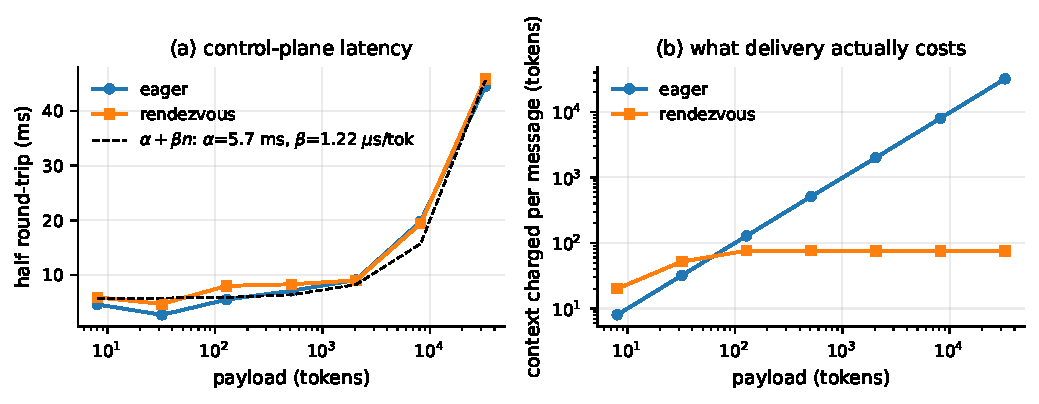
\includegraphics[width=\columnwidth]{figures/fig_latency}
\caption{Control-plane latency and context cost versus payload size. The
eager/rendezvous crossover is visible in (b): rendezvous charges the receiver an
envelope regardless of payload size.}
\label{fig:latency}
\end{figure}

\paragraph{Collective volume confirms the analysis.} \Cref{fig:collvolume} plots
messages and payload tokens against $P$. Ring allgather performs $P(P-1)$
messages (\agRingMsgs at $P=\collMaxP$) and moves \agRingTokens tokens against
recursive doubling's \agRdMsgs messages and \agRdTokens tokens, a factor of
\agRingRatio. Dissemination barrier performs $P\lceil\log_2 P\rceil$ messages and
linear $2(P-1)$, both exactly as predicted. The \op{flat} family performs zero
messages at every $P$, which is the control-plane observation of
\Cref{sec:asymmetries} made concrete.

\begin{figure*}[t]
\centering
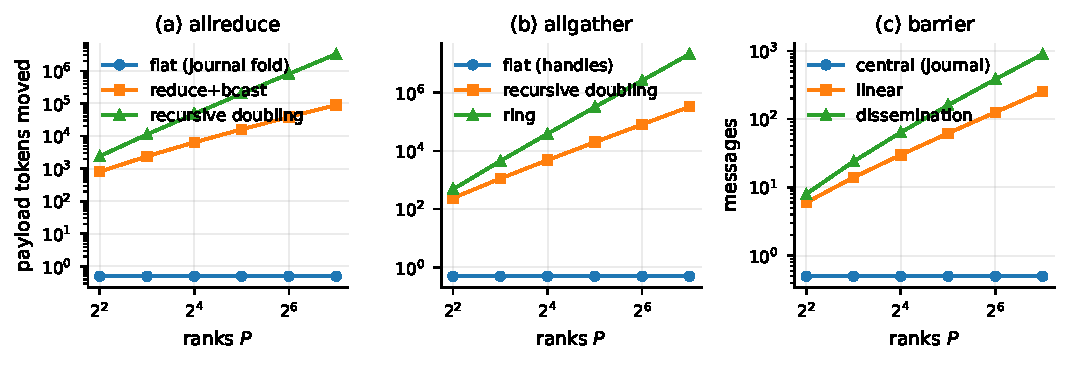
\includegraphics[width=\textwidth]{figures/fig_collective_volume}
\caption{Collective cost versus $P$. Journal-mediated (\op{flat}) schedules move
no messages at all; the tree and ring schedules reproduce their textbook message
and volume complexities.}
\label{fig:collvolume}
\end{figure*}

\paragraph{MPI's short-message optimum is the wrong choice for agent operators.}
At $P=\collMaxP$, recursive-doubling allreduce performs \arRdMsgs messages moving
\arRdTokens payload tokens, against reduce-then-broadcast's \arRbMsgs messages and
\arRbTokens tokens: \textbf{\arRdRatio$\times$ the data volume}. In MPI that extra
volume is worth paying because it removes a broadcast phase and the redundant
arithmetic is free. Under \Cref{eq:cost} the arithmetic is not free and the volume
is charged to context, so the ranking inverts. This is the paper's clearest
demonstration that the catalogue transfers but the selection rule must be
rederived.

\paragraph{Agent-operator reduction depth.} With a simulated
$\gamma = \mergeCostS$\,s (\Cref{fig:agentreduce}), a binomial tree at
$P=\agentRedP$ gives the busiest executor \agentRedBinMaxPerRank merges ---
matching $\lceil\log_2 P\rceil$ exactly at all \agentRedBinPoints measured points
--- and completes in \agentRedBinWall\,s, against the linear chain's
\agentRedChainWall\,s: a speedup of \agentRedSpeedup$\times$ at identical total
work (\agentRedBinTotal applications either way). The chain's serialised depth is
$P-1=\agentRedChainDepth$ even though each rank performs one merge, which is
exactly the distinction between per-rank work and dependency depth.

\begin{figure}[t]
\centering
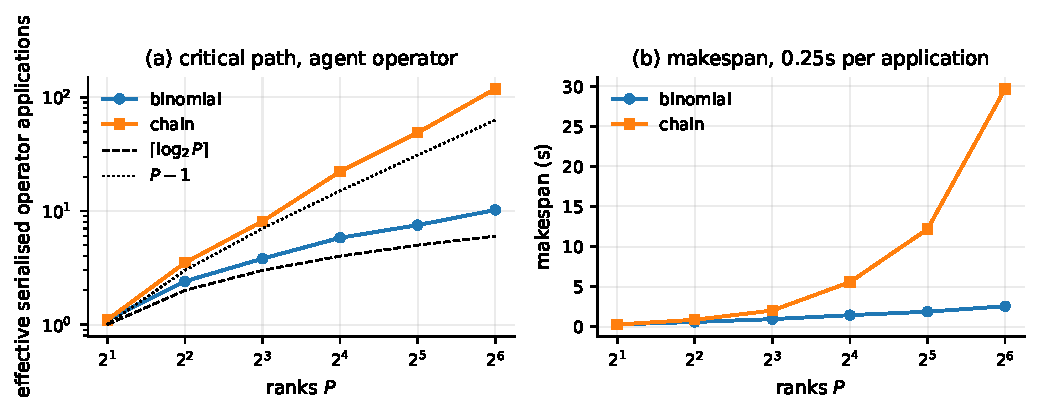
\includegraphics[width=\columnwidth]{figures/fig_agent_reduce}
\caption{Agent-evaluated reduction. (a) effective serialised operator
applications; (b) makespan at $\gamma=\mergeCostS$\,s. Total work is identical;
only the dependency depth differs.}
\label{fig:agentreduce}
\end{figure}

\paragraph{Context cost is where the protocol earns its keep.}
\Cref{fig:context} and \Cref{tab:context} report tokens delivered into context
windows at $P=\ctxP$ with \ctxPayloadTokens-token payloads. An allgather that
inlines bodies charges one rank \ctxAgInlinePeak tokens --- far beyond any
context window --- and \ctxAgInlineTotal across the job. Handle-based delivery
charges that rank \ctxAgHandlePeak and \ctxAgHandleTotal in total:
\ctxAgPeakRatio$\times$ and \ctxAgTotalRatio$\times$ reductions respectively.
Broadcast shows the same effect at smaller magnitude
(\ctxBcInlineTotal $\rightarrow$ \ctxBcHandleTotal). Bounded views sit between the
two, trading fidelity for a fixed per-contribution cost. This is the concrete
mechanism behind ``context exhaustion'' in agent harnesses, and it is a
flow-control choice rather than an inevitability.

\begin{table}[t]
\centering
\small
\begin{tabular}{@{}llrr@{}}
\toprule
Collective & Delivery & Total tokens & Peak in one rank \\
\midrule
\multirow{3}{*}{bcast}
 & inline  & \ctxBcInlineTotal & \ctxBcInlinePeak \\
 & handle  & \ctxBcHandleTotal & \ctxBcHandlePeak \\
 & view (400) & \ctxBcViewTotal & \ctxBcViewPeak \\
\midrule
\multirow{3}{*}{allgather}
 & inline  & \ctxAgInlineTotal & \ctxAgInlinePeak \\
 & handle  & \ctxAgHandleTotal & \ctxAgHandlePeak \\
 & view (400) & \ctxAgViewTotal & \ctxAgViewPeak \\
\bottomrule
\end{tabular}
\caption{Tokens entering agent context windows, $P=\ctxP$,
\ctxPayloadTokens-token payloads.}
\label{tab:context}
\end{table}

\begin{figure}[t]
\centering
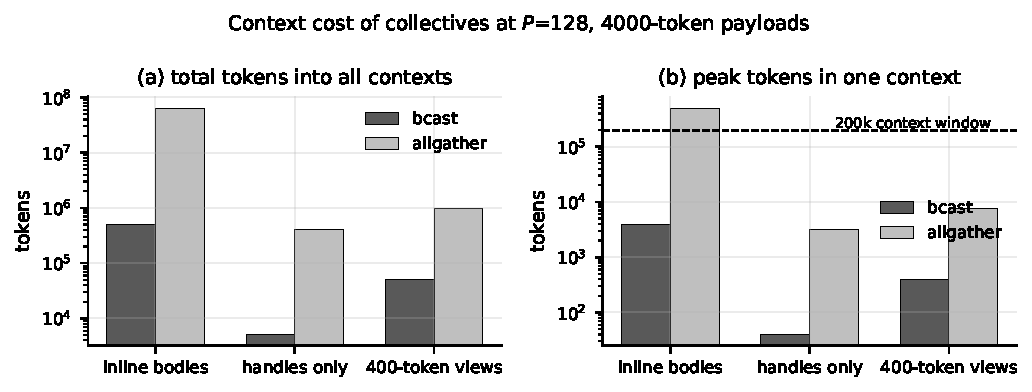
\includegraphics[width=\columnwidth]{figures/fig_context}
\caption{Context cost by delivery discipline. The dashed line marks a
200\,k-token context window: inlined allgather exceeds it by more than
$2\times$ at $P=\ctxP$.}
\label{fig:context}
\end{figure}

\paragraph{Matching does not degrade with queue depth.} Receive latency is flat
from an empty unexpected queue (\matchMedianEmpty\,ms) to \matchMaxDepth queued
messages (\matchMedianDeep\,ms). MPI implementations pay a linear scan of the match
list, and several studies measure the cost; an indexed durable match list does
not, which is a concrete benefit of the journal-as-network choice rather than an
assertion about it.

\paragraph{Barrier crossover.} \Cref{fig:barrier} shows the journal-mediated
barrier beating a dissemination tree at $P=\barPMid$
(\barCentralMid\,s vs.\ \barDissemMid\,s) and losing at $P=\barPHigh$
(\barCentralHigh\,s vs.\ \barDissemHigh\,s); the crossover lies between 32 and
64, which is the measurement behind the selection threshold in
\Cref{sec:selection}. The shared medium behaves like a
switch with in-network aggregation up to a point and like a contended resource
past it --- the same reason MPI implementations abandon linear collectives at
scale.

\begin{figure}[t]
\centering
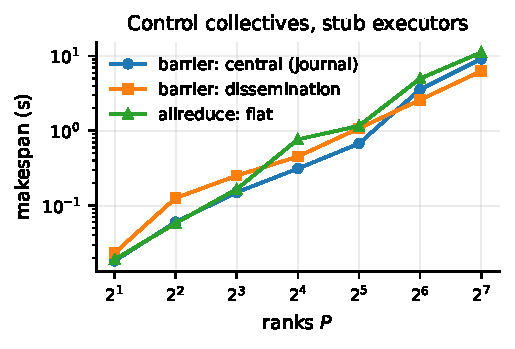
\includegraphics[width=\columnwidth]{figures/fig_barrier_scaling}
\caption{Control collectives with stub executors. The shared medium is not free
at scale.}
\label{fig:barrier}
\end{figure}

\subsection{Multi-agent applications}
\label{sec:eval:apps}

Each rank below is a separate LLM agent with its own context window, launched
with a prompt containing its identity, its assignment and the protocol manual.
Agents coordinate \emph{only} through \cli{ampi}; there is no shared conversation
and no orchestrator reading their output.

\paragraph{Arms are ablations, not strawmen.} Every application runs twice. The
\op{naive} arm has the same agents, the same task, the same assignment and the
same shared filesystem, and still uses \ampi for identity, launch and metering ---
it simply uses it the way a harness written without the protocol's discipline
does: no negotiated agreement, no boundary exchange, and a final gather that
materialises full bodies. Comparing against a baseline that also lacked
instrumentation would produce numbers we could not interpret.

\subsubsection{E1: parallel book translation}
\label{sec:eval:e1}

Translation looks embarrassingly parallel, and a naive harness scales trivially.
What makes it a real parallel programming problem is that the pieces are not
independent: two translators who never talk render invented terminology
differently, and section $i+1$ does not follow from how section $i$ ended. The
dependencies are a \emph{global agreement} (terminology) and a
\emph{nearest-neighbour agreement} (boundaries) --- precisely the two dependency
structures MPI exists to express, namely a reduction and a halo exchange.

Corpus: Abbott's \emph{Flatland} (1884, public domain), which is unusually dense
in invented vocabulary that must be rendered consistently (Flatland, Lineland,
Regularity, Chief Circle, the Colour Bill). Target: Simplified Chinese. Each rank
owns one section. The \ampi arm performs (i) \op{AMPI\_Scatter} of assignments,
(ii) \op{AMPI\_Allreduce} with an \emph{agent} operator to reconcile per-section
terminology proposals into one glossary, (iii) translation using that glossary,
(iv) a halo exchange over a 1-D Cartesian topology in which each rank sends its
closing sentences downstream and revises its opening, and (v) handle-based
\op{AMPI\_Gather}. The \op{naive} arm omits (ii) and (iv) and materialises bodies
in (v).

\emph{Metric.} For each probe term we take the rendering each rank reports having
actually used and compute the share held by the modal rendering among ranks whose
section contains that term. A term rendered identically everywhere scores 1.0;
three renderings among three ranks scores 0.33. Glossary adherence is checked
against the \emph{collective's own result object} in the journal, not against
anything an agent claimed, because a protocol that agrees a value nobody then uses
has bought nothing. Boundary revision is read from window cell versions, which is
durable evidence rather than self-report.

\emph{Results.} \Cref{tab:e1} reports both arms at $P=\eOneAmpiP$. Both
completed every section, in statistically indistinguishable wall time
(\eOneNaiveWall\,s vs.\ \eOneAmpiWall\,s) and with comparable output volume, so
the protocol arm's coordination cost did not show up as latency. What differs is
the artefact and the context.

Of \eOneAmpiTermsScored probe terms reported by two or more ranks, the
unprotocolled arm diverged on two --- \emph{Equilateral} was rendered two ways in
a two-two split, and \emph{Priest} two ways by two ranks --- giving a mean modal
share of \eOneNaiveModal and \eOneNaiveFullyConsistent of terms fully
consistent. The \ampi arm diverged on none: mean modal share \eOneAmpiModal, all
terms consistent. The agreed glossary contained \eOneGlossaryTerms terms, produced
by \eOneMergeTotal agent-evaluated merges with \eOneMergeCrit on the critical
path --- matching $\lceil\log_2 P\rceil$ --- and adherence to it, checked against
the collective's own result object rather than against agent self-report, was
\eOneAdherence. The halo exchange caused \eOneRevised of \eOneAmpiP ranks to
revise and republish their opening (a window-cell version above one), against
none in the unprotocolled arm.

Peak context in a single rank was \eOneNaivePeakCtx tokens against
\eOneAmpiPeakCtx --- a factor of \eOnePeakCtxRatio --- because the unprotocolled
arm's coordinator materialised every translation while the \ampi arm's collected
handles.

\emph{How much to conclude.} This is one run per arm at $P=\eOneAmpiP$ with
\eOneAmpiTermsScored scored terms, so the terminology effect rests on two
divergences. We report it as a demonstration that the mechanism does what it is
supposed to do --- the glossary was agreed, adherence was total, and the
divergences the unprotocolled arm exhibited are exactly the ones a glossary
prevents --- and not as an effect size. The context result is not
sample-limited: it is a structural consequence of handle-based collection and
matches \Cref{tab:context}.

\begin{table}[t]
\centering
\small
\begin{tabular}{@{}lrr@{}}
\toprule
& no protocol & \ampi \\
\midrule
ranks & \eOneNaiveP & \eOneAmpiP \\
sections completed & \eOneNaiveCompletion & \eOneAmpiCompletion \\
mean modal share & \eOneNaiveModal & \eOneAmpiModal \\
fully consistent terms & \eOneNaiveFullyConsistent & \eOneAmpiFullyConsistent \\
distinct renderings/term & \eOneNaiveDistinct & \eOneAmpiDistinct \\
peak context (tokens) & \eOneNaivePeakCtx & \eOneAmpiPeakCtx \\
total context (tokens) & \eOneNaiveTotalCtx & \eOneAmpiTotalCtx \\
timeout retries & \eOneNaiveRetries & \eOneAmpiRetries \\
\bottomrule
\end{tabular}
\caption{E1, parallel book translation. Glossary adherence in the \ampi arm was
\eOneAdherence over \eOneGlossaryTerms agreed terms, produced by \eOneMergeTotal
agent-evaluated merges with \eOneMergeCrit on the critical path.}
\label{tab:e1}
\end{table}

\subsubsection{E2: collaborative software development}
\label{sec:eval:e2}

Software development is the tightly-coupled case, and it is hard in the way
tightly-coupled parallel codes are hard: the pieces depend on each other mutually,
the interfaces between them are not given in advance, and a disagreement about a
shared representation does not degrade the result --- it produces something that
does not run.

Eight agents implement MiniScheme, a Scheme interpreter in Python: reader, value
representation and printer, environments and closures, special forms, evaluator
with proper tail calls, and three primitive modules, plus an integrator. The
\emph{public} behaviour is fixed by a specification; the \emph{internal}
interfaces --- how a pair is represented, what an environment lookup returns for
an unbound name, how a special form hands a tail expression back to the evaluator
--- are deliberately unspecified. Agreeing them is the coordination problem.
Grading is by a \eTwoSuite-case held-out suite the agents never see, run
per-case in a fresh subprocess with a wall-clock limit, so a module that loops
forever costs one test rather than the run.

The \ampi arm reduces eight interface proposals into one contract with an agent
operator, publishes it in a window, keeps an append-only decisions log written
with lock-free \op{accumulate}, takes a leased lock around the single genuinely
shared file, and runs two synchronised integration rounds separated by
\op{Win\_fence} and \op{Barrier} with test failures distributed by
\op{AMPI\_Bcast}. The \op{naive} arm has the same eight agents, the same
specification and module assignment, and a shared filesystem they may read freely
--- a strong baseline, since a shared repository with no coordination protocol is
how most multi-agent coding harnesses actually work.

\begin{figure}[t]
\centering
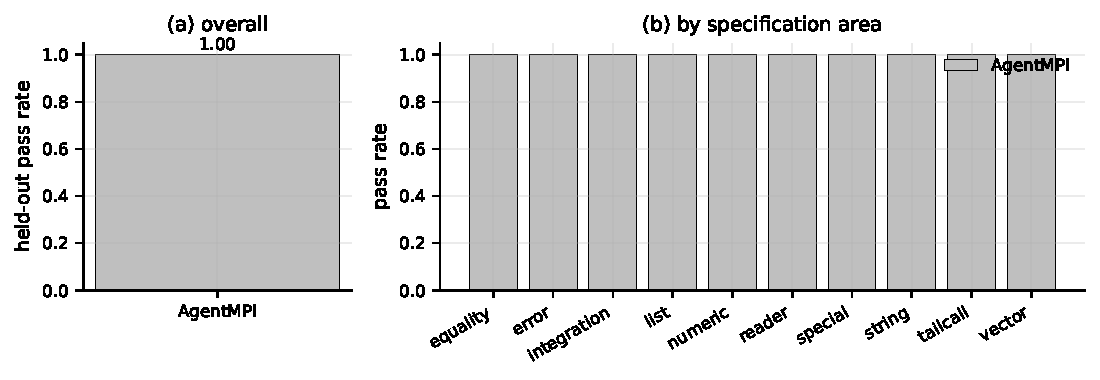
\includegraphics[width=\columnwidth]{figures/fig_e2}
\caption{E2. Both arms passed every held-out case, so (a) carries no
information; (b) and (c) do. The unprotocolled arm created more window cells and
sent more point-to-point messages than the protocol arm --- it built its own
coordination layer --- while the protocol arm's prescribed contract phase
accounts for almost all of its extra cost.}
\label{fig:e2}
\end{figure}

\emph{Results: a null result, and a more interesting one behind it.} Both arms
passed \textbf{\eTwoAmpiPass of \eTwoSuite} held-out cases --- every case, in every
category, in both arms --- having also each passed all 43 visible smoke tests. The
negotiated contract made no difference to the outcome. We report that plainly
because it is what happened, and then we report what the journals show about
\emph{why}, which we think is the more useful finding.

\paragraph{The unprotocolled arm invented the protocol.} The \op{naive} arm's
program gave it no coordination phase: no contract, no decisions log, no
synchronised rounds. Its agents nonetheless created \eTwoNaiveWindows windows of
their own accord, containing cells named \op{interface}, \op{eval-protocol},
\op{datum-expectations}, \op{rank05-primitives}, \op{rank03.env} and
\op{integration-status}, and exchanged \eTwoNaivePtp point-to-point messages ---
against the \ampi arm's \eTwoAmpiPtp. Given the primitives and a problem that
needs agreement, they reached for a shared contract in a window and per-rank
interface declarations: that is, for very nearly the structure the protocol
prescribes.

We find this more persuasive than a pass-rate difference would have been. A
pass-rate difference shows that one harness beat another harness. Eight agents
independently converging on ``publish a contract into shared state, declare what
you provide, message the owner when you need a change'' is evidence that the
abstraction matches the shape of the problem. It is also a caution: the
mechanisms are not the protocol's contribution --- being able to \emph{specify}
them, name them, and see them afterwards is.

\paragraph{The prescribed process was expensive.} \Cref{tab:e2} and
\Cref{fig:e2} give the cost.
The \ampi arm took \eTwoAmpiWall\,s against \eTwoNaiveWall\,s
(\eTwoWallRatio$\times$), made \eTwoAmpiCalls runtime calls against
\eTwoNaiveCalls, and delivered \eTwoAmpiCtx tokens into agent contexts against
\eTwoNaiveCtx (\eTwoCtxRatio$\times$). Almost all of that is the phase our harness
imposed: agree a complete contract by agent-evaluated reduction \emph{before}
anyone writes code, then two synchronised integration rounds. On this task that
was wasted work.

The honest reading is that this is a harness design error, not a protocol result.
The \op{naive} arm used the same primitives opportunistically --- publish an
interface when you have one, read a peer's when you need it --- and got the same
artefact for a third of the wall time. A harness author with these primitives
should prefer that, and reach for the full contract reduction only when
opportunistic agreement demonstrably fails.

\begin{table}[t]
\centering
\small
\begin{tabular}{@{}lrr@{}}
\toprule
& no protocol phase & \ampi \\
\midrule
held-out cases passed & \eTwoNaivePass & \eTwoAmpiPass \\
pass rate & \eTwoNaiveRate & \eTwoAmpiRate \\
\midrule
wall time (s) & \eTwoNaiveWall & \eTwoAmpiWall \\
runtime calls & \eTwoNaiveCalls & \eTwoAmpiCalls \\
tokens into contexts & \eTwoNaiveCtx & \eTwoAmpiCtx \\
point-to-point messages & \eTwoNaivePtp & \eTwoAmpiPtp \\
window cells created & \eTwoNaiveCells & \eTwoAmpiCells \\
lock-free accumulates & \eTwoNaiveAcc & \eTwoAmpiAcc \\
agent-evaluated merges & 0 & 7 \\
interpreter lines written & \eTwoNaiveLines & \eTwoAmpiLines \\
\bottomrule
\end{tabular}
\caption{E2, eight ranks per arm, graded by a \eTwoSuite-case held-out suite. The
quality outcome is identical; the cost is not. The unprotocolled arm created its
own contract and decisions windows without being asked to.}
\label{tab:e2}
\end{table}

\paragraph{Why the task did not discriminate.} Three conditions made agreement
easy, and each identifies where we would expect the result to change. The agents
\emph{shared a filesystem}, so a rank could read its dependency's source instead
of asking about it --- remove that and the negotiated contract becomes the only
channel. The public specification \emph{pinned the observable behaviour
tightly}, leaving the internal representations underdetermined but strongly
suggested. And the artefact was a Scheme interpreter, about which current models
hold strong shared priors: a \op{Pair} class with mutable fields, primitives in a
dict, a trampoline for tail calls. A task with genuinely novel internal
interfaces, or eight ranks that cannot see each other's files, is where we would
expect the contract to earn its cost. We did not run that experiment.

\paragraph{What the run does establish.} \Cref{tab:e2mech} audits the mechanisms
under real agent load, which is worth having independently of the comparison. The
reduction tree's shape is the cleanest check: rank 0 performed exactly
$\lceil \log_2 8\rceil = 3$ merges, rank 4 performed 2, ranks 2 and 6 one each,
and no other rank performed any --- the binomial schedule, $P-1 = 7$ applications
in total, executed by eight independent agents over 46 minutes with no shared
context. The contract it produced was 21\,638 tokens, published once as a window
cell; inlining it to eight ranks would have cost 173\,104 tokens of context
against the 21\,638 one handle-based publication costs.

\begin{table}[t]
\centering
\footnotesize
\begin{tabularx}{\columnwidth}{@{}l r X@{}}
\toprule
\textbf{Mechanism} & \textbf{Count} & \textbf{Reading} \\
\midrule
agent merges (contract) & 7 & $P-1$, with 3 on rank 0: the binomial schedule exactly \\
contract size & 21\,638 tok & published once as a window cell, not broadcast \\
decisions-log writes & 31 & lock-free \op{accumulate}: no rank serialised on a lock to record a decision \\
fix-log writes & 19 & two synchronised integration rounds \\
lock acquisitions & 8 & the one genuinely shared source file \\
timeout retries & \eTwoAmpiTimeouts & every one resumed the same wait; none abandoned \\
peak context per rank & 12.1--22.1k tok & against a 140k budget \\
\bottomrule
\end{tabularx}
\caption{E2 mechanism evidence under real agent load, from the journal.}
\label{tab:e2mech}
\end{table}

The \eTwoAmpiTimeouts timed-out calls deserve a sentence. Every one was a rank
waiting for a peer that was still writing code, and every one resumed rather than
restarted, because the internal-retry default of \Cref{sec:deadlines} made
persistence the runtime's responsibility. In the pilot run that motivated that
default, the same situation ended with an executor abandoning a collective after
two timeouts.

\subsubsection{E3: mass launch failure}
\label{sec:eval:e3}

Our agent host enforces a limit of ten concurrent background agents. A run
requested at $P=\eThreeRequestedP$ therefore started only \eThreeStartedP ranks,
and the remaining \eThreeNeverStarted never called \op{AMPI\_Init}. Rather than
discard it we let it proceed, because a \eThreeFailureRatePct\% launch failure
exercises the whole of \Cref{sec:ft} at once and does so with none of the
artificiality of injected faults: nobody chose which ranks would fail, when, or in
what state.

The run \textbf{completed}. All \eThreeFinalized surviving ranks finalised, and
\eThreeCollsClosed of \eThreeCollsTotal collectives closed --- the assignment
scatter, the agent-evaluated glossary allreduce, the result gather, a numeric
allreduce and the final barrier --- with \eThreeDeclaredFailed of
\eThreeRequestedP ranks declared failed. The survivors produced
\eThreeSections complete translated sections in the shared window, in
\eThreeWall\,s. \Cref{tab:e3} audits which mechanism fired.

\begin{table}[t]
\centering
\small
\begin{tabularx}{\columnwidth}{@{}l X@{}}
\toprule
\textbf{Mechanism} & \textbf{Evidence from the journal} \\
\midrule
Join deadline (\Cref{sec:ft}) & \eThreeNeverStarted ranks that never called
\op{AMPI\_Init} were detected and declared failed. Without a lease granted at
request time they would have been neither alive nor failed, and every collective
would have waited forever. \\
Fault-tolerant reduction tree & \eThreeSubtreesDropped dead subtrees dropped; the
agent-evaluated glossary allreduce closed on the survivors' contributions after
\eThreeMerges agent merges. \\
Local failure notification & 4 \op{AMPI\_ERR\_PROC\_FAILED} returns, each raised
at the rank that happened to be waiting on a dead peer --- not broadcast. \\
Deadline-bounded blocking & 6 \op{AMPI\_ERR\_TIMEOUT} returns, all resumed by
re-issuing the identical call. \\
Fencing (\Cref{sec:design}) & 1 \op{AMPI\_ERR\_FENCED}: a rank declared failed
after a long silent step was stopped rather than allowed to keep publishing into a
job that had written it off. \\
Quorum collectives & the final barrier released on the survivors and closed in
4.2\,s. \\
\bottomrule
\end{tabularx}
\caption{E3 audit. Every row is read from the journal, not from an agent's
report.}
\label{tab:e3}
\end{table}

The single \op{AMPI\_ERR\_FENCED} is the episode that motivated two-phase
detection (\Cref{sec:ft}). One surviving translator went silent for 580\,s of
legitimate work --- it had been instructed to extend its lease before long steps
and did not --- and the single-phase detector in use at the time convicted it.
Conviction is terminal by design, so the rank could not finish what it had. Under
the two-phase detector now specified, that silence would have raised suspicion
without redistributing its work, and its next call would have cleared it.

\emph{What this run does and does not show.} It is a demonstration of graceful
degradation, not a measurement of it: we did not choose the failure pattern, so we
cannot report recovery cost as a function of failure rate. What it does establish
is that the mechanisms compose --- join deadlines, local notification, subtree
dropping, fencing and quorum release all fired in one run, unrehearsed, and the
job produced a coherent partial artefact instead of hanging or aborting. For a
first evaluation of a fault-tolerance design that is the property we most wanted
to check, because the usual failure of such designs is that each primitive works
in isolation and they deadlock together.

\subsection{Status of the experimental results}
\label{sec:status}

Every number in this paper is generated from a results file rather than typed,
and a claim whose measurement is absent fails the build instead of going stale.
At the time this draft was generated:

\begin{itemize}
\item \textbf{Complete}: all microbenchmarks (\Cref{sec:eval:micro}); E1 both
arms at $P=\eOneAmpiP$; E2 both arms at $P=8$, each graded against the full
\eTwoSuite-case held-out suite; the E3 fault-tolerance audit.
\item \textbf{Not attempted}: application runs above $P=8$; a task with genuinely
novel internal interfaces or without a shared filesystem, which
\Cref{sec:eval:e2} argues is where the E2 comparison would discriminate.
\end{itemize}

\Cref{sec:threats} discusses the threats to validity, of which the most serious
is identity drift in the agent host.

The harnesses, the grading suite, the probe-term list and the analysis scripts are
all in the artefact, and \texttt{scripts/reproduce.sh} regenerates everything that
does not require an agent host and prepares the launch plans for what does.

\subsection{Threats to validity}
\label{sec:threats}

\paragraph{Identity drift contaminated every run.} As \Cref{tab:drift} records,
the host's shared shell sessions caused stray \op{AMPI\_Init} calls in four of
five runs. We report the affected results anyway, for three reasons, and readers
should weigh them. First, the contamination is \emph{auditable}: every window
write and message records its writer's rank and epoch, so the artefacts we score
are attributed from the journal rather than from what an agent claimed. Second,
re-initialising a running rank is a heartbeat rather than a new epoch, so a stray
\op{init} did not displace its victim; the agents detected the drift, pinned their
identity, and completed their assigned work. Third, the E1 metrics are computed
from window cells whose writer field matches the intended rank, and the E2
grading runs against the source tree, which is owned per-file. The exception is
E3, where drift and genuine launch failure are partly confounded: some ranks that
appear failed had agents running under another rank's identity for part of the
run. We therefore present E3 as a demonstration that the mechanisms compose, not
as a measurement of failure rate, which is how \Cref{sec:eval:e3} already framed
it.

\paragraph{Single runs.} Every application result is one run per arm. Agent runs
are expensive and our concurrency ceiling was ten, so we have no variance
estimates. Where an effect is small we decline to claim it; where it is
structural --- context cost, schedule shape, message counts --- it does not depend
on sampling.

\paragraph{Application scale.} The concurrency ceiling bounded real-agent runs at
$P=8$, well below the microbenchmark range. The selection thresholds in
\Cref{sec:selection} are validated with stub executors, not agents.

\paragraph{Our harnesses had bugs, and they are in the results.} Three of the
fourteen lessons in \Cref{sec:lessons} are defects in the experiment harnesses
rather than in the protocol: a conditional send against an unconditional receive
(L9), a round-two tag mismatch, and a prescribed schedule far heavier than the
task needed (L10). These cost wall time and one operator intervention, all
disclosed. We report them because a paper that presented only the runs that went
smoothly would be describing a different protocol from the one we built.

%======================================================================
\section{What only real agents exposed}
\label{sec:lessons}

Several protocol defects were invisible to a unit test suite and to stub
executors, and appeared the first time real agents ran the protocol. We report
them because they are the paper's most transferable content.

\paragraph{L1. Executors give up far earlier than instructed.} Told to retry a
timed-out call up to twenty times, a rank stopped after two and stalled its whole
reduction tree. The fix is not a better prompt: blocking operations now retry
internally by default, so persistence is the runtime's responsibility and
abandoning a collective requires the executor to do something rather than
nothing.

\paragraph{L2. Blocking is not evidence of death.} An early runtime had ranks make
no calls while waiting inside a collective, so the lease-based detector declared
each rank that arrived \emph{first} to be dead, and the job cascaded --- a 12-rank
demonstration took 94\,s with every barrier timing out. Making the progress engine
renew the caller's lease, run the detector and observe revocation took the same run
to 8.9\,s with all survivors recovering. A blocked rank has obligations.

\paragraph{L3. Executors do not volunteer liveness.} Given an explicit lease
extension primitive and an explicit instruction to call it before long steps, an
agent did not, and was declared dead mid-translation. Since being declared dead is
terminal, the detector must not depend on cooperation: hence two-phase detection,
and hence the launcher --- which actually knows whether a process exists --- as the
authority for immediate conviction.

\paragraph{L4. Program order is not a reliable collective identifier.} Agents
retry commands, skip steps and reorder independent calls. Identifying a collective
by position silently mismatches ranks. Explicit labels were the single largest
robustness improvement we made.

\paragraph{L5. A rank that never starts must still be detectable.} See
\Cref{sec:eval:e3}: without a lease granted at request time, a no-show is neither
alive nor failed.

\paragraph{L6. Quorum must release without closing.} Closing a barrier on reaching
quorum guarantees that precisely the slowest ranks fail. Straggler-tolerant
synchronisation has to let latecomers through.

\paragraph{L7. Errors must prescribe.} Agents act on a hint naming the next
command far more reliably than they infer a remedy from a description of the
fault. This is why every \ampi error carries a hint and why retryable errors say
so in their own output.

\paragraph{L8. Ambient identity without an assertion is unsafe, and we had to be
shown.} An earlier draft of \Cref{sec:design} argued that making rank ambient
``eliminates the entire class'' of wrong-rank errors. It eliminated the error we
designed against --- agents \emph{passing} the wrong rank --- and replaced it with
a worse one: agents silently \emph{being} the wrong rank. Our agent host shares
shell sessions between concurrently running agents, so \op{AMPI\_RANK} was
overwritten between one call and the next. The journals record the consequence
exactly: in each of four independent runs, one specific rank accumulated
\emph{eight or nine} \op{AMPI\_Init} events, one from nearly every other agent in
the job (\Cref{tab:drift}). Every agent's first \op{init} ran as somebody else.
In one run it escalated: the victim's own calls were credited elsewhere, its
lease starved, and it was declared failed and fenced while actively working.

Nineteen of twenty-two agents reported this independently, and every one reached
the same workaround --- prefix the identity inline on every invocation --- because
the interface offered nothing better. It now does: \op{--expect-rank} and
\op{--expect-job} fail with \op{AMPI\_ERR\_IDENTITY} before the operation runs, an
explicit root argument overrides the environment variable, every command echoes
the identity it acted as, and the launcher issues a per-rank token that the
runtime checks --- so a drifted rank is told which rank it actually holds
credentials for. Ambient identity remains the default, because an agent forced to
thread its rank through every call will get \emph{that} wrong instead. What
changed is that asserting it is now possible and cheap.

Two design decisions limited the damage and are worth requiring of any
implementation. Re-initialising a rank that is already \emph{running} is treated
as a heartbeat rather than a new epoch, so a stray \op{init} did not fence its
victim. And every window write and message records its writer's rank and epoch,
so the corruption was auditable afterwards --- which is how we can quantify it at
all rather than merely suspecting it.

\begin{table}[t]
\centering
\small
\begin{tabular}{@{}llr@{}}
\toprule
Run & Ranks & \op{init} events on the drift target \\
\midrule
E1 (P=22, launch failure) & 22 & 8 on rank 2 \\
E1b, protocol arm (P=5)   & 5  & 0 \\
E1b, ablated arm (P=5)    & 5  & 9 on rank 4, 2 on rank 3 \\
E2, protocol arm (P=8)    & 8  & 8 on rank 1 \\
E2, ablated arm (P=8)     & 8  & 8 on rank 7 \\
\bottomrule
\end{tabular}
\caption{Identity drift, from the journals. One rank per run absorbed a stray
\op{AMPI\_Init} from nearly every other agent, because the host's shell sessions
were shared and one agent's exported \op{AMPI\_RANK} leaked into the others.
Because window writes and messages record their writer, the contamination is
auditable rather than merely suspected.}
\label{tab:drift}
\end{table}

\paragraph{L9. Never truncate an operand.} A reduction operand is the input to a
function, so removing part of it does not degrade the result, it corrupts it ---
and for structured payloads it is worse, because clipping JSON mid-string yields
a document the operator cannot parse. We shipped the naive behaviour and it bit
immediately: agents serving as internal nodes received operands cut mid-string
with an elision marker spliced in, and independently invented recovery hacks, one
prefix-matching the content-addressed object store by hand, another reordering
its output so the decisions it could not afford to lose came before the part
clipping would take. The asymmetry to respect is that a \emph{result} may be
summarised, because its consumer is a reader; an \emph{operand} may not, because
its consumer is a function.

\paragraph{L10. Print only commands that exist.} Our reduction directive told the
agent to run a subcommand spelled with a space where the real one is hyphenated.
Roughly ten agents reported it, several while peers were blocked behind them. A
binding that prints a command an agent cannot copy-paste is worse than one that
prints nothing, because the agent trusts it.

\paragraph{L11. Give every payload a free path to disk.} Agents that wanted to
keep a large result without paying context for it reached into the object store
directly, or paid. Both are our fault: every operation that hands back a payload
needs an option to write it to disk, since nothing enters a context window that
way.

\paragraph{L12. An interface invites a process; do not confuse the two.} Our E2
harness prescribed the heaviest schedule the interface allows --- agree a complete
contract by agent-evaluated reduction before writing any code, then two
synchronised integration rounds --- and it cost \eTwoWallRatio$\times$ the wall
time and \eTwoCtxRatio$\times$ the context of an arm that used the same primitives
opportunistically, for the same result. Having a collective for agreement does not
mean agreement should be a phase. The mistake is ours, not the protocol's, but it
is the mistake a protocol makes easy, and it is worth naming: prefer opportunistic
publication, and escalate to a full reduction only when it demonstrably fails.

\paragraph{L13. A conditional send plus an unconditional receive is a deadlock,
and the protocol cannot save you from it.} Our own E2 harness contained this bug.
The integrator was told to send a fix assignment \emph{for each failure}; the
other ranks were told to receive one. When the test suite passed, there were no
failures, so four ranks sat in a receive that nobody would ever satisfy. This is
the oldest bug in message passing and \ampi does not prevent it --- no interface
can, because the mistake is in the program. What it did do is worth recording:
the deadline-bounded receive turned an unbounded hang into a stall that
\cli{ampi status} localised in one command, naming the four ranks missing from
the barrier and the exact tag they were waiting on; and because the receives
remained posted, the ranks were recoverable rather than lost. The harness lesson
is the same one MPI teaches about collectives with zero-length buffers:
\emph{send unconditionally, possibly empty}. An empty assignment is still an
assignment.

\paragraph{L14. Schema evolution is a live concern.} Adding a column to the journal
mid-experiment broke a running 22-rank job. A durable protocol store must migrate
on open; a journal written by an older runtime has to stay readable.

%======================================================================
\section{Discussion and limitations}
\label{sec:discussion}

\paragraph{Does this argue for more agents?} No, and our own E2 result argues
against over-claiming. The strongest objection to multi-agent systems is that
splitting work disperses context and decision-making, and that one agent holding
everything often does better. We think that objection is largely right, and that
it is an argument about \emph{mechanism}: it holds when the only tools available
are ad-hoc message passing and prompt concatenation. \ampi is a claim about what
changes when information sharing, agreement and recovery are first-class --- not a
claim that more agents are better.

E2 sharpens this. Eight agents produced a working system either way, and the arm
we ablated recreated the protocol's mechanisms by itself. What the protocol bought
there was not capability but \emph{legibility}: after the run we can say how many
operator applications the agreement took, in what tree, what the contract cost in
tokens, which rank held which lock, and that 46 timed-out calls resumed rather
than failed. That is worth something to a harness author, and it is much less than
we would have claimed had the pass rates differed. It also tells us the honest
scope of the contribution: \ampi is for harnesses whose coordination you need to
be able to specify and audit, not for proving that coordination is necessary.

\paragraph{Scale of the real-agent runs.} A ten-concurrent-agent ceiling on our
host bounded real-agent $P$ well below the microbenchmark range. This is a
limitation of the evaluation, not of the design, but it is a real one: we cannot
report a 128-agent application run, and the selection thresholds in
\Cref{sec:selection} are validated with stub executors. It is also the standard
shape of an HPC evaluation --- microbenchmarks at scale, applications at the scale
the machine allows --- and we have been explicit about which claims rest on which.

\paragraph{Silent failure is not solved.} A5 includes plausible-but-wrong output,
and \ampi provides only mechanism for it: redundancy through \op{vote}, selection
through \op{maxby}, attribution through window writer records. Detecting that a
result is wrong remains the harness's problem, as ABFT leaves verification to the
algorithm~\cite{huang1984abft}. We regard a protocol that claimed to solve it as
overreaching.

\paragraph{The token is an imperfect unit.} Thresholds denominated in tokens make
the eager/rendezvous decision estimator-dependent, so two implementations may
classify the same payload differently. This affects cost, not correctness, and we
require implementations to report their estimator --- but a protocol whose central
threshold is approximate is worth flagging.

\paragraph{What we deliberately omitted.} Following MPI's practice of standardising
only what is understood: automatic context compaction policy, semantic
verification, cost-aware scheduling, inter-communicators, persistent collectives,
partitioned communication, sessions, and capability discovery. Each is a research
question, and a standard that answers one prematurely is worse than one that leaves
a hook.

%======================================================================
\section{Related work}
\label{sec:related}

\paragraph{Classical agent communication languages.} KQML~\cite{finin1994kqml} and
FIPA-ACL~\cite{fipa2002acl} standardised \emph{speech acts} with mentalistic
semantics. They achieved little durable adoption, and the critiques are
instructive: the semantics were unverifiable from observable behaviour, and the
ontology commitment raised the cost of participation. \ampi takes MPI's opposite
bet. What those systems got right and modern systems have largely lost is
explicitness about interaction structure --- FIPA's Contract
Net~\cite{smith1980contractnet} is a named, analysable protocol in a way that
``the orchestrator delegates to workers'' is not --- and \ampi's labelled
collectives and declared topologies are an attempt to recover exactly that.
Blackboard systems~\cite{erman1980hearsay} anticipate our windows, and their
central difficulty, control, is what \op{Win\_fence} addresses. Tuple
spaces~\cite{gelernter1985linda} anticipate associative matching; MPI's explicit
addressing won in HPC for locality reasons that apply here too.

\paragraph{Modern agent protocols.} MCP~\cite{mcp2026spec} standardises the
agent-to-tool boundary; A2A~\cite{a2a2026site} the agent-to-agent \emph{task}
boundary. Both are valuable and neither is a competitor: they occupy the transport
and single-peer-delegation layers, and provide no group membership, no
collectives, no consistency model for shared state and no failure model. \ampi
sits above them and could be carried over either.

\paragraph{Orchestration frameworks.} AutoGen~\cite{wu2023autogen},
LangGraph~\cite{langgraph2026guide}, CrewAI and the OpenAI Agents SDK are
frameworks: they supply a coordination pattern (conversation, graph, crew,
handoff) and the application is written inside it. LangGraph's checkpointers and
durable execution overlap our recovery briefing, and AutoGen's actor rewrite
overlaps our mailboxes. The difference is the same one that separated MPI from the
frameworks of its era: a framework owns control flow, an interface does not. Our
gather-returns-a-manifest rule and context ledger have, to our knowledge, no
counterpart.

\paragraph{Research multi-agent systems.} MetaGPT~\cite{hong2024metagpt} defines a
publish-subscribe message pool and standardised outputs;
ChatDev~\cite{qian2024chatdev} a chat chain over a waterfall process;
CAMEL~\cite{li2023camel} role-playing dialogue. Each embeds a coordination
mechanism in an application. Multi-agent debate~\cite{du2023debate} and
self-consistency~\cite{wang2023selfconsistency} are, in our terms, allreduce with
\op{vote}; best-of-$n$ is allreduce with \op{maxby}. That these fall out as
operator choices rather than as architectures is some evidence the abstraction is
at the right level. The MAST taxonomy~\cite{cemri2025mast} of multi-agent failures
maps closely onto the failure classes of \Cref{sec:ft}.

\paragraph{Parallel programming models.} We borrow bulk synchrony from
BSP~\cite{valiant1990bridging} for window epochs, bounded staleness from
SSP~\cite{ho2013ssp} for quorum collectives, lineage-based recovery from
Spark~\cite{zaharia2012rdd} and durable execution for the recovery briefing,
distributed object stores from Ray~\cite{moritz2018ray} for handles, and
supervision trees from OTP~\cite{armstrong2003thesis}. We chose two-sided message
passing plus one-sided windows over pure actors because actors have no collectives
and no group naming, and over pure dataflow because agent work is not a static
graph.

\paragraph{Context management.} MemGPT~\cite{packer2023memgpt} treats the context
window as virtual memory to be paged, and PagedAttention~\cite{kwon2023pagedattention}
does the analogous thing for KV cache; both are OS analogies, where ours is a
network one. Views are closer to derived datatypes than to paging: the harness
declares which projection it wants rather than relying on a policy to evict.
Long-context degradation~\cite{liu2024lostmiddle} is a further argument for
delivering less rather than more.

%======================================================================
\section{Conclusion}

MPI's history suggests that the way out of a proliferation of incompatible
coordination layers is a thin, mechanism-level interface with a reference
implementation, not another framework. We have tried to carry that answer into
multi-agent systems, and found that MPI's structure transfers almost intact while
its cost model does not. Denominating transfer cost in tokens turns context
exhaustion into flow control; making the reduction operator an agent makes
serialised operator applications the dominant cost and inverts MPI's algorithm
selection in at least one standard case; and treating individual, frequent,
sometimes-silent failure as normal requires ULFM plus leases, fencing epochs, join
deadlines and replacement briefings. Two findings are, we suspect, more durable than the design. The first is the
catalogue of defects that only real agents exposed: executors abandon retries, do
not volunteer liveness, and cannot be trusted to keep program order. Each is an
argument about where responsibility for reliability has to sit, and the answer is
never the agent. The second is our own null result. Eight agents given these
primitives but told nothing about how to coordinate built a contract window and
per-rank interface declarations by themselves, and matched the prescribed
schedule's output for a third of its cost. That the abstraction is what agents
reach for is the best evidence we have that it is the right abstraction; that they
reach for it unprompted is a warning against selling it as a capability. What a
protocol offers is not that coordination becomes possible, but that it becomes
something a harness author can state, bound, and afterwards read back.

\bibliographystyle{plain}
\bibliography{refs}

\balance
\end{document}
